\documentclass[12pt, a4paper]{classes/exam}
\usepackage{array}
\usepackage{tikz}
\usepackage{circuitikz}
\usepackage{siunitx}
\usepackage{array}
\usepackage{multicol}
\usepackage{multirow}
\usepackage{graphicx}
\usepackage{physics}
\graphicspath{ {./images/} }
\usepackage{wrapfig}
\usepackage[table]{xcolor}
\usepackage{multicol}
\usepackage{pdflscape}
\usepackage{adjustbox}
\usepackage{pdfpages}
\usepackage{tkz-euclide}
\definecolor{myyellow}{RGB}{254,241,24}
\definecolor{myorange}{RGB}{234,125,1}
\definecolor{fancyorange1}{RGB}{253,138,9}
\definecolor{fancyorange2}{RGB}{246,156,123}
\usepackage{tkz-euclide}
\usetikzlibrary{quotes,arrows.meta}
\usepackage{makecell}
\begin{document}
	\begin{figure}[H]
		\centering
		\begin{tikzpicture}
		\node at (0,0) {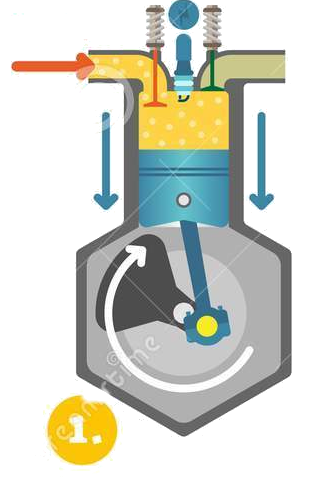
\includegraphics[scale=7]{first_strokes}};
		\end{tikzpicture}
	\end{figure}
	\begin{figure}[H]
		\centering
		\begin{tikzpicture}
		\node at (0,0) {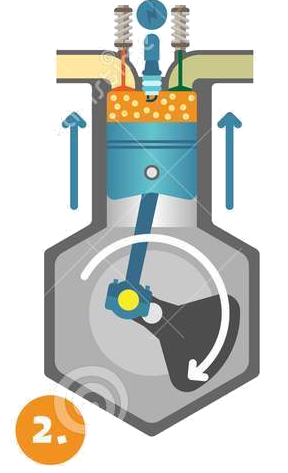
\includegraphics[scale=7]{second_strokes}};
		\end{tikzpicture}
	\end{figure}
	\begin{figure}[H]
		\centering
		\begin{tikzpicture}
		\node at (0,0) {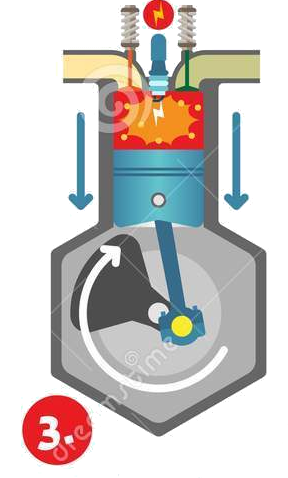
\includegraphics[scale=7]{third_strokes}};
		\end{tikzpicture}
	\end{figure}
	\begin{figure}[H]
		\centering
		\begin{tikzpicture}
		\node at (0,0) {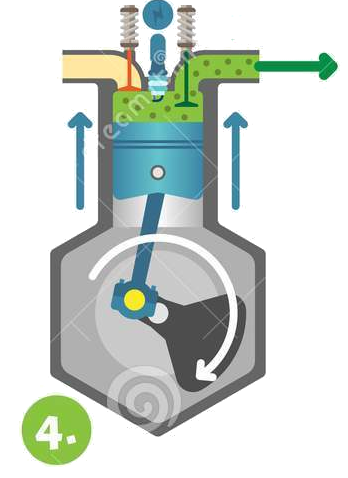
\includegraphics[scale=7]{four_strokes}};
		\end{tikzpicture}
	\end{figure}
\end{document}